%----------------------------------------------------------------------------------------
%	PACKAGES AND OTHER DOCUMENT CONFIGURATIONS
%----------------------------------------------------------------------------------------

\documentclass[twoside]{article}

\usepackage{lipsum} % Package to generate dummy text throughout this template
\usepackage{algorithm}
\usepackage{algpseudocode}
\usepackage[sc]{mathpazo} % Use the Palatino font
\usepackage[T1]{fontenc} % Use 8-bit encoding that has 256 glyphs
\linespread{1.05} % Line spacing - Palatino needs more space between lines
\usepackage{microtype} % Slightly tweak font spacing for aesthetics

\usepackage[hmarginratio=1:1,top=32mm,columnsep=20pt]{geometry} % Document margins
\usepackage{multicol} % Used for the two-column layout of the document
% Custom captions under/above floats in tables or figures
\usepackage[hang, small,labelfont=bf,up,textfont=it,up]{caption}
\usepackage{booktabs} % Horizontal rules in tables
\usepackage{float}
\usepackage{hyperref} % For hyperlinks in the PDF

\usepackage{lettrine}
\usepackage{paralist}

\usepackage{abstract} % Allows abstract customization
\renewcommand{\abstractnamefont}{\normalfont\bfseries} % Set the "Abstract" text to bold
\renewcommand{\abstracttextfont}{\normalfont\small\itshape} % Set the abstract itself to small italic text

\usepackage{titlesec} % Allows customization of titles
\renewcommand\thesection{\Roman{section}} % Roman numerals for the sections
\renewcommand\thesubsection{\Roman{subsection}} % Roman numerals for subsections
\titleformat{\section}[block]{\large\scshape\centering}{\thesection.}{1em}{}
\titleformat{\subsection}[block]{\large}{\thesubsection.}{1em}{}

\usepackage{fancyhdr} % Headers and footers
\pagestyle{fancy} % All pages have headers and footers
\fancyhead{} % Blank out the default header
\fancyfoot{} % Blank out the default footer
\fancyhead[C]{ESE650 Learning in Robotics $\bullet$ April 2014 $\bullet$ Project 5}
\fancyfoot[RO,LE]{\thepage} % Custom footer text

\usepackage[pdftex]{graphicx}
\usepackage{epstopdf}
\usepackage{subfigure}
\usepackage{amsmath,amssymb,amsopn,amstext,amsfonts}
\usepackage{url}
\usepackage[usenames,dvipsnames]{color}
\usepackage{siunitx}
\usepackage{amsmath}
\usepackage{amsfonts}
\usepackage{amssymb}

\graphicspath{{fig/}}
\newcommand{\W}{\mathcal{W}}
\newcommand{\X}{\mathcal{X}}
\newcommand{\Y}{\mathcal{Y}}
\newcommand{\Z}{\mathcal{Z}}
\newcommand{\red}[1]{\textcolor{red}{#1}}
\newcommand{\brown}[1]{\textcolor{brown}{#1}}

%-------------------------------------------------------------------------------
%	TITLE SECTION
%-------------------------------------------------------------------------------

\title{\vspace{-15mm}\fontsize{24pt}{10pt}\selectfont\textbf{Cost Learning and Path Planning}} % Article title

\author{
\large
\textsc{Chao Qu}\thanks{A thank you or further information}\\[2mm] % Your name
\normalsize University of Pennsylvania \\ % Your institution
\normalsize \href{mailto:quchao@seas.upenn.edu}{quchao@seas.upenn.edu} % Your email address
\vspace{-5mm}
}
\date{}

%-------------------------------------------------------------------------------

\usepackage{graphicx}
\begin{document}


\maketitle % Insert title

\thispagestyle{fancy} % All pages have headers and footers

%-------------------------------------------------------------------------------
%	ABSTRACT
%-------------------------------------------------------------------------------

%\begin{abstract}
%
%\noindent Hey, I'm just an abstract. % Dummy abstract text
%
%\end{abstract}

%-------------------------------------------------------------------------------
%	ARTICLE CONTENTS
%-------------------------------------------------------------------------------

%-------------------------------------------------------------------------------
%	INTRODUCTION
%-------------------------------------------------------------------------------

\begin{multicols}{2} % Two-column layout throughout the main article text

\section{Introduction}
\lettrine[nindent=0em,lines=2]{P}ath planning problems have been long studied in robotics. Planning algorithms rely on fully specified cost map that are usually manually designed and programmed. In this project, we are trying to let the robot 'learn' a cost map with examples demonstrated by human. This is called imitation learning. Here we use the LEARCH framework to learn a cost function for planning based on an aerial satellite image of the Penn campus.

%-------------------------------------------------------------------------------
%	PRE-PROCESSING
%-------------------------------------------------------------------------------

\section{Pre-processing}
%-------------------------------------------------------------------------------
%	METHODS
%-------------------------------------------------------------------------------
Since the provide image is very big, we first subsample the image and then smooth it with a median filter to remove noise while preserve edges. After that, we crop the image to a bunch of small tiles for training and testing. We train strictly on training set and test on the test set. 
We use a class MDP to represent a single training/test data. The MDP class consists of the original image, a feature matrix, loss field and a policy (or path). 
For the feature matrix, we use the following features (might change in final submission)
\begin{enumerate}
\item binary mask of black and white pixels
\item binary mask of red and green pixels
\item probability of the pixel being vegetation, road, roof and sidewalk
\item edge from matlab canny edge
\end{enumerate}
We append all these features together to generate a feature matrix. This feature matrix multiplied by a linear function will give us a cost map.
As for loss field, we use something similar to Hamming loss, which has typically 0 along the example and 1 away from the example path. The intuition of such loss field can be found in the LEARCH paper. A sample loss field can be seen in Fig.

\section{Methods}
For the training part, we strictly follow the algorithm from the paper, which is algorithm 5 \textbf{Exponentiated functional gradient descent for maximum margin planning}.
For the regressor, we chose l2-loss l2-regularized logistic regression from liblinear with a cost parameter of 0.1. If time allow we will play with this parameter or with different classifiers or regressors.
Since the LEARCH algorithm doesn't specify a convergence criteria, here we just use $T=25$ and adjust the learning rate so that it decreases with iteration.

%-------------------------------------------------------------------------------
%	RESULTS
%-------------------------------------------------------------------------------

\section{Results}
Here we show some results with our learning algorithm. In all the following plot, the images have never been seen by the learner.
The blue lines are human drawn example path just for reference, and purple lines are actual learned path. We see from the test results that the learner learned the human demonstrated path pretty well.
Below are some tests of walking
\begin{figure}[H]
\centering
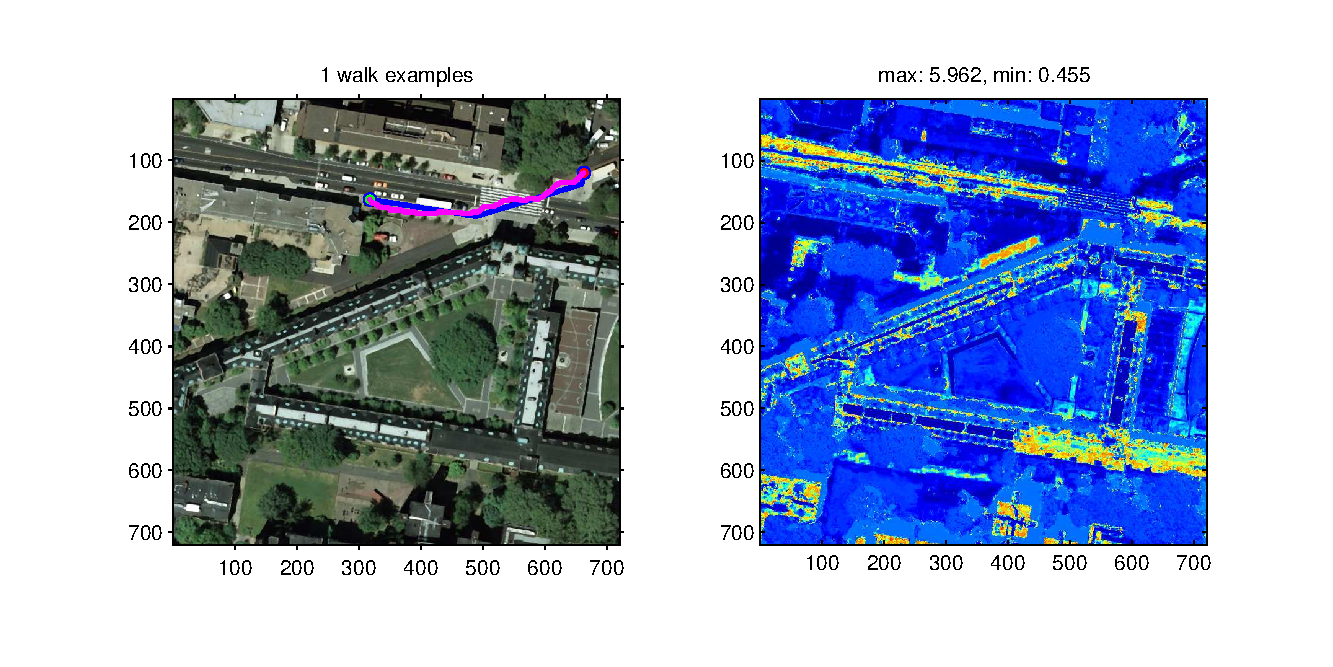
\includegraphics[width=\columnwidth]{fig/walk1.pdf}
\caption{walk1}
\label{fig:walk1}
\end{figure}

\begin{figure}[H]
\centering
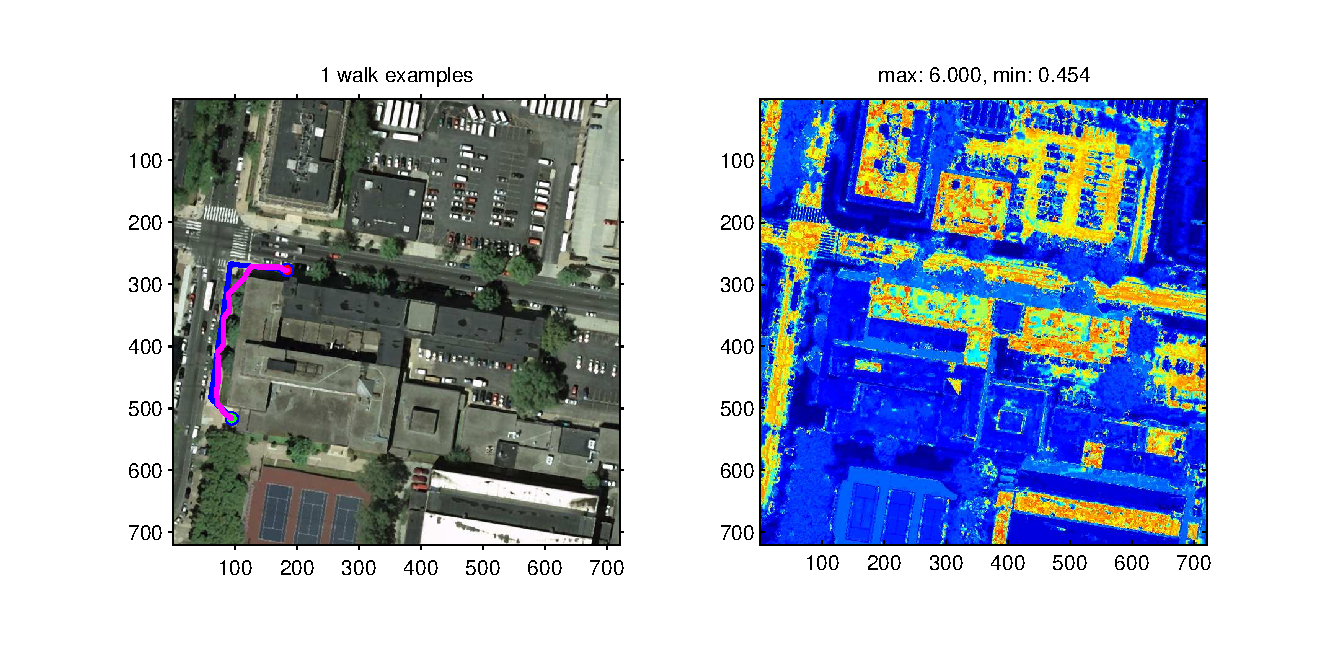
\includegraphics[width=\columnwidth]{fig/walk2.pdf}
\caption{walk2}
\label{fig:walk2}
\end{figure}

\begin{figure}[H]
\centering
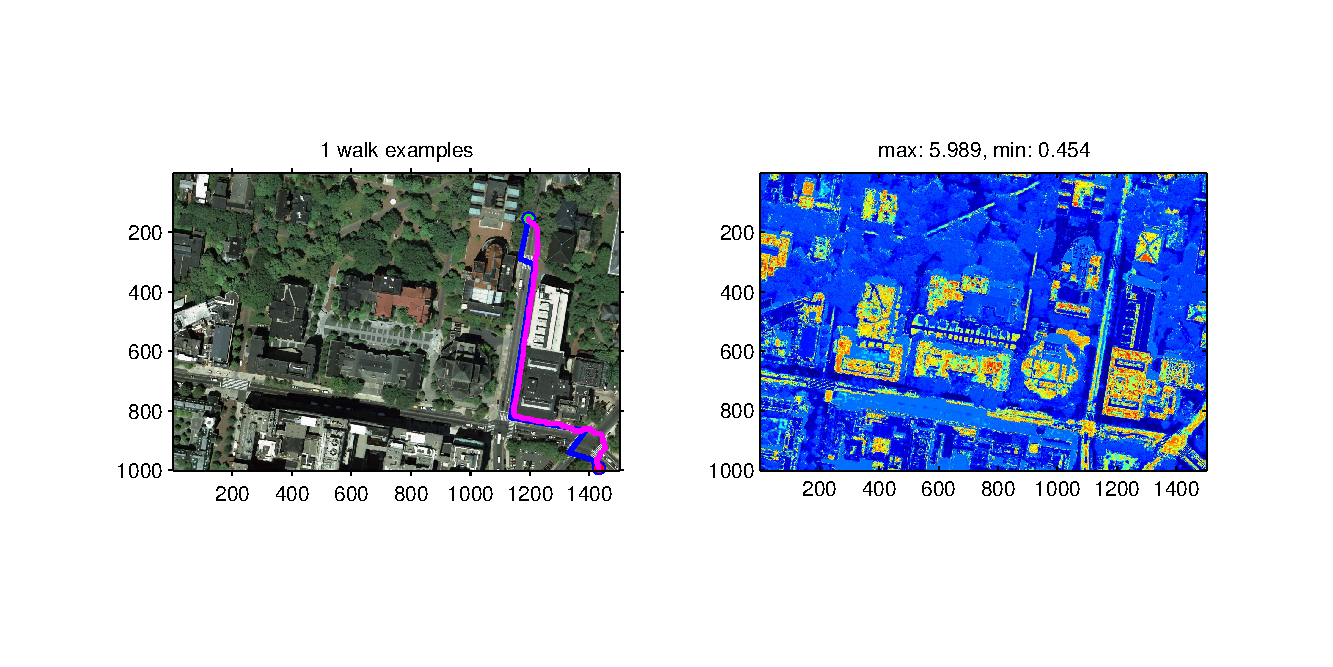
\includegraphics[width=\columnwidth]{fig/walk3.pdf}
\caption{walk3}
\label{fig:walk3}
\end{figure}

\begin{figure}[H]
\centering
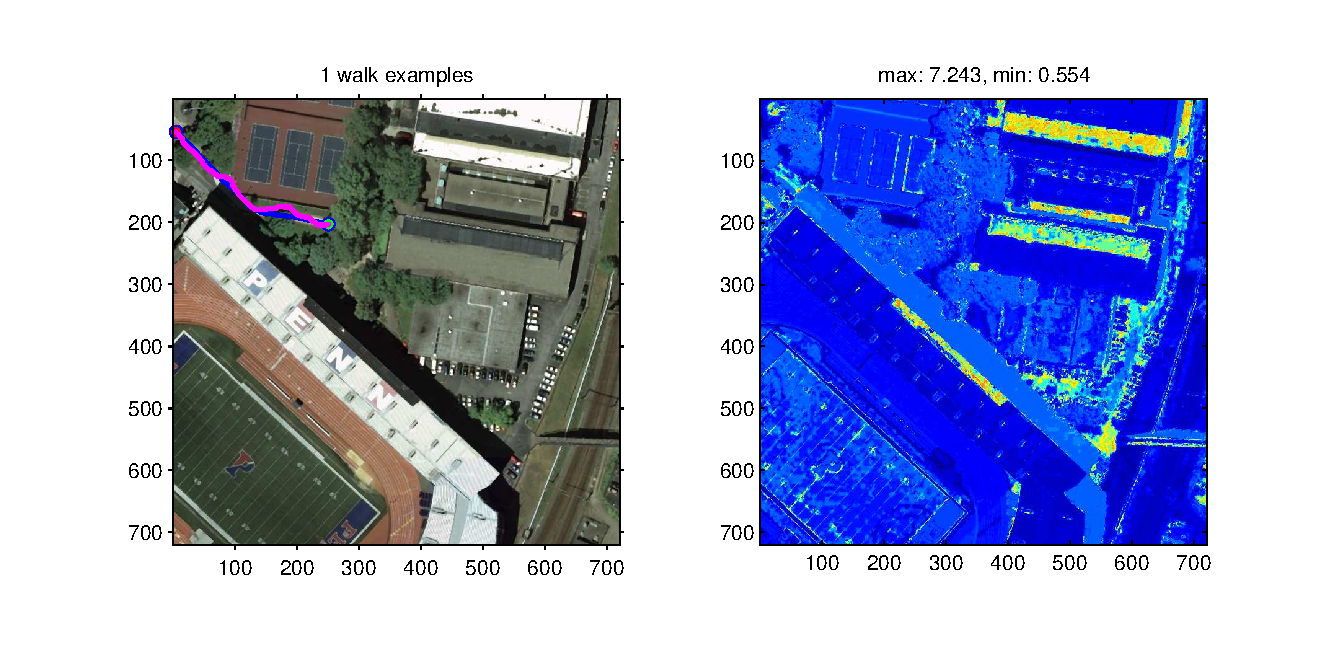
\includegraphics[width=\columnwidth]{fig/walk4.pdf}
\caption{walk4}
\label{fig:walk4}
\end{figure}

\begin{figure}[H]
\centering
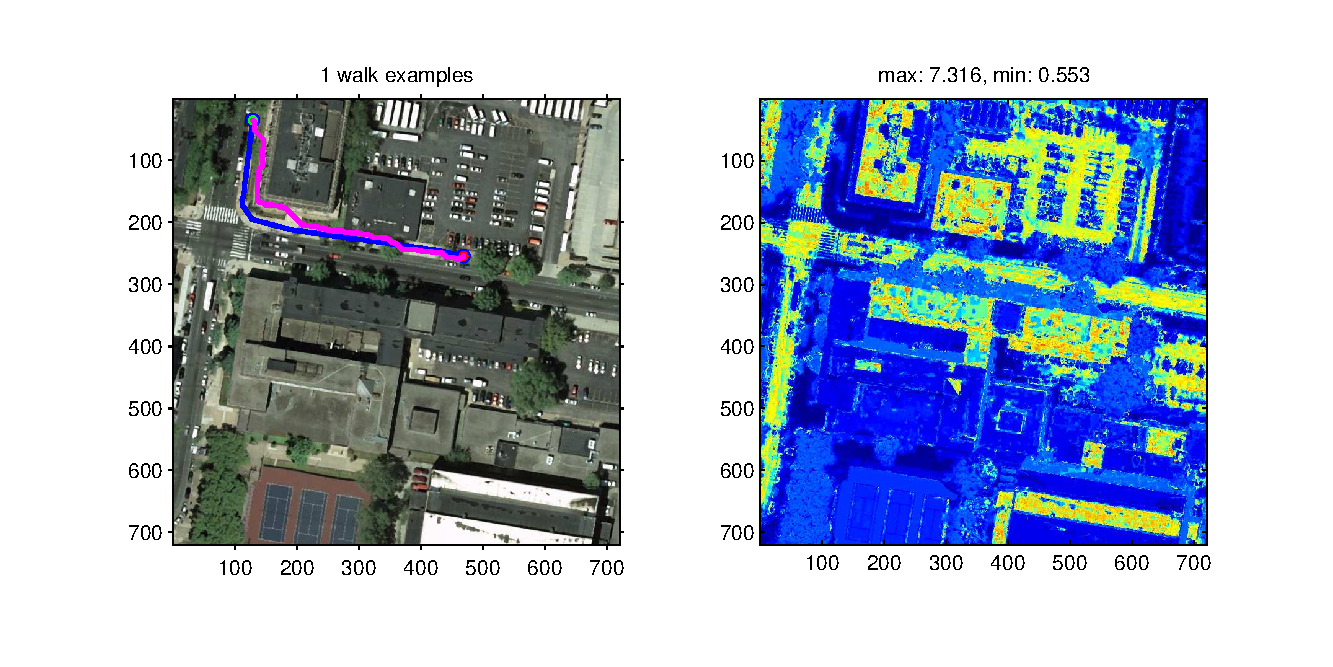
\includegraphics[width=\columnwidth]{fig/walk5.pdf}
\caption{walk5}
\label{fig:walk5}
\end{figure}

\begin{figure}[H]
\centering
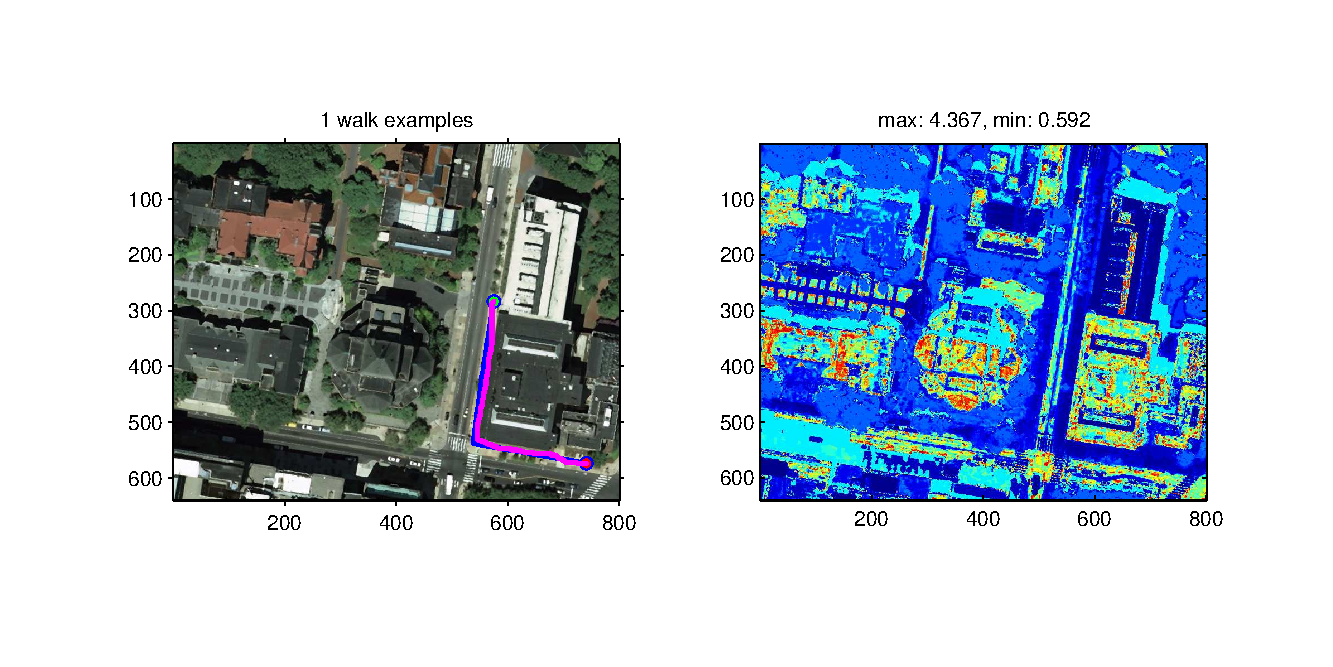
\includegraphics[width=\columnwidth]{fig/walk6.pdf}
\caption{walk6}
\label{fig:walk6}
\end{figure}

\begin{figure}[H]
\centering
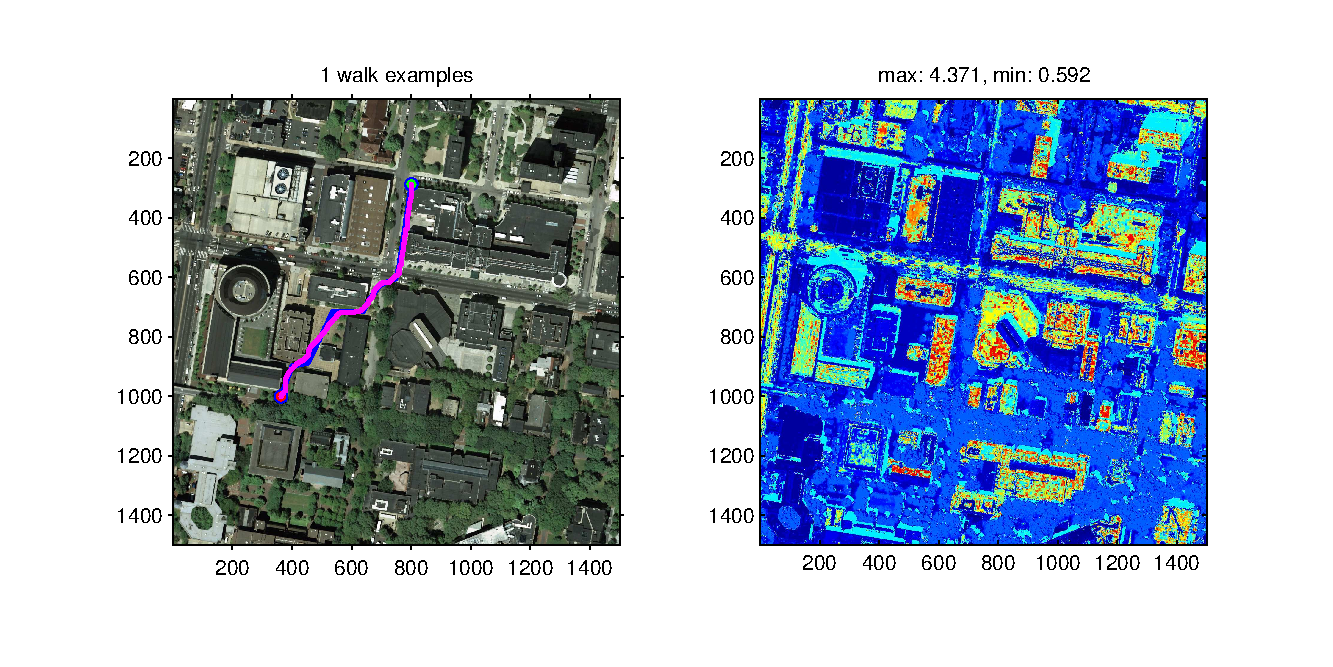
\includegraphics[width=\columnwidth]{fig/walk7.pdf}
\caption{walk7}
\label{fig:walk7}
\end{figure}


Here are some tests of driving
\begin{figure}[H]
\centering
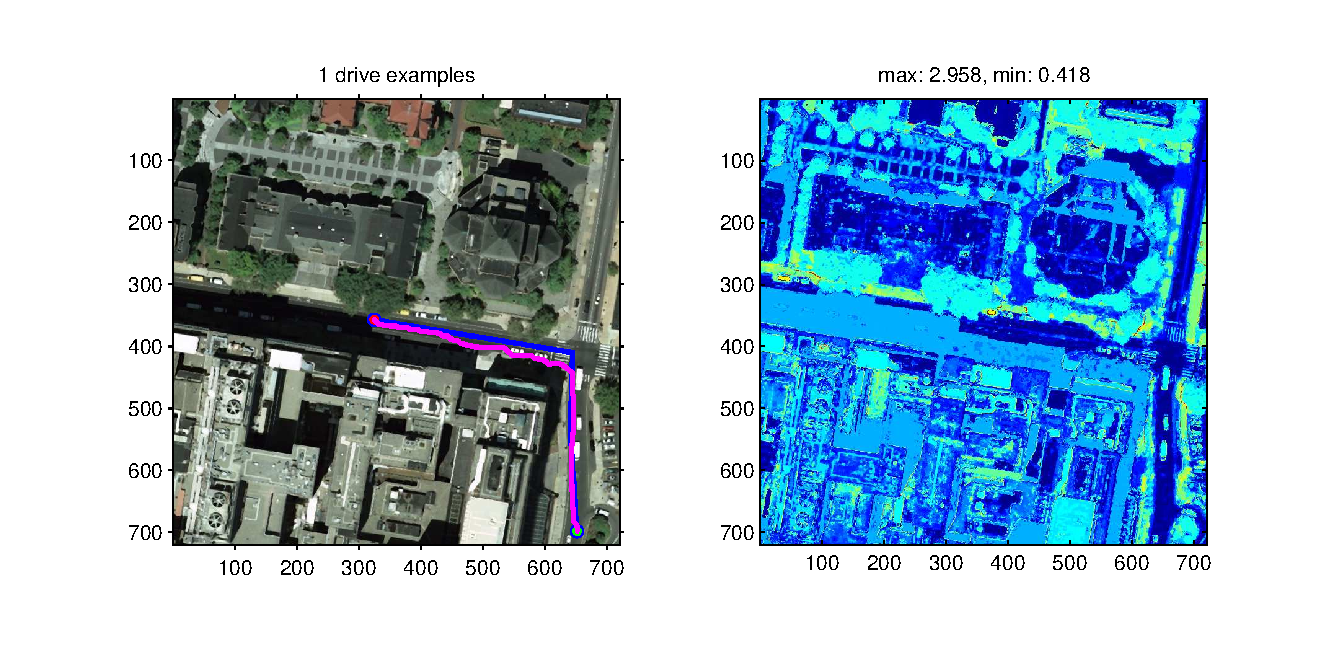
\includegraphics[width=\columnwidth]{fig/drive1.pdf}
\caption{drive1}
\label{fig:drive1}
\end{figure}

\begin{figure}[H]
\centering
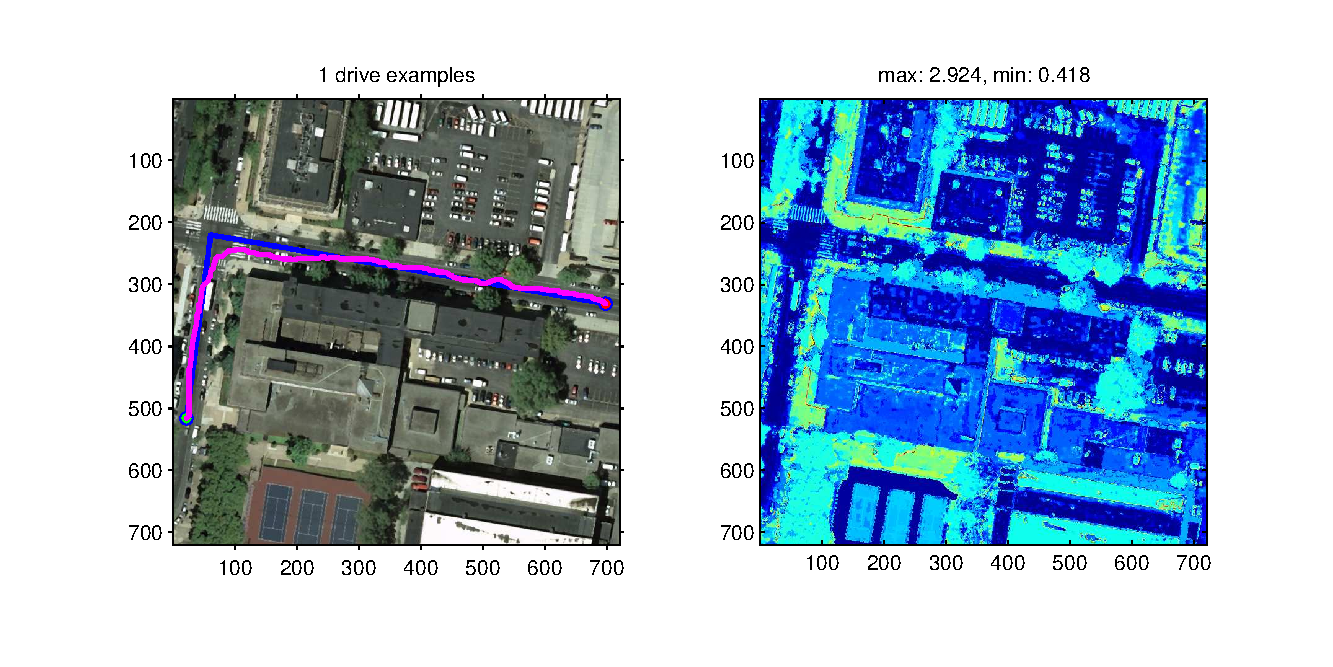
\includegraphics[width=\columnwidth]{fig/drive2.pdf}
\caption{drive2}
\label{fig:drive2}
\end{figure}

\begin{figure}[H]
\centering
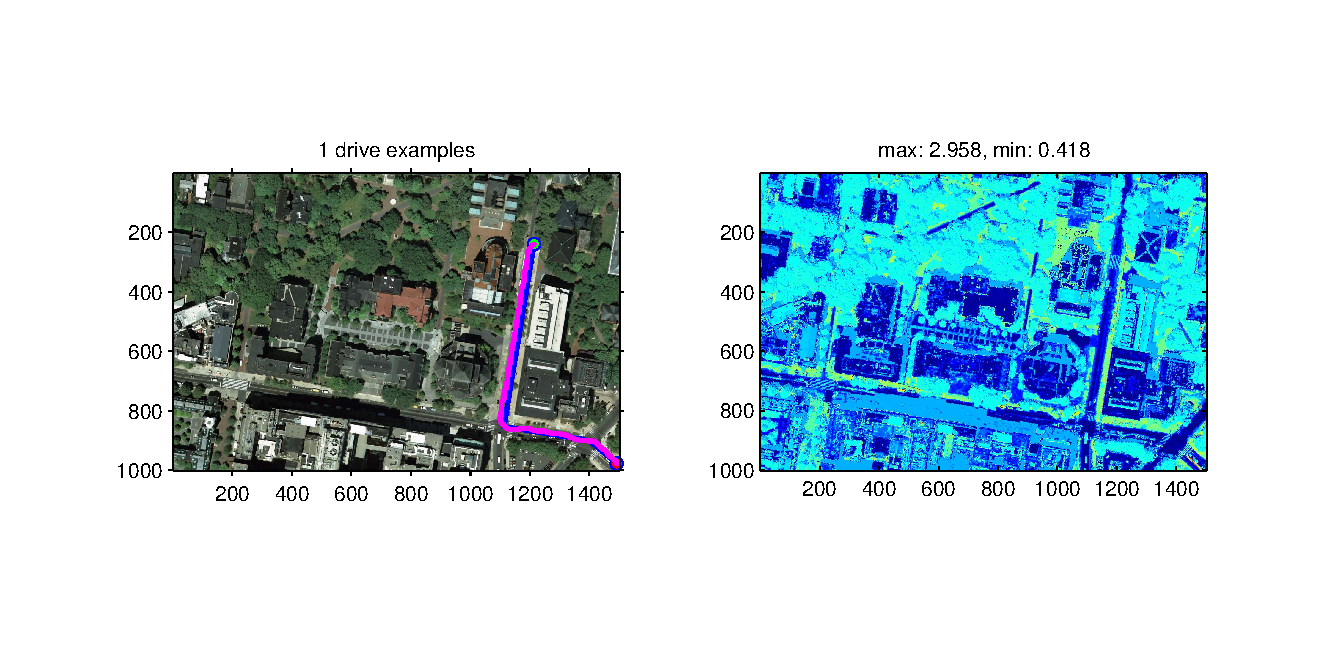
\includegraphics[width=\columnwidth]{fig/drive3.pdf}
\caption{drive3}
\label{fig:drive3}
\end{figure}

\begin{figure}[H]
\centering
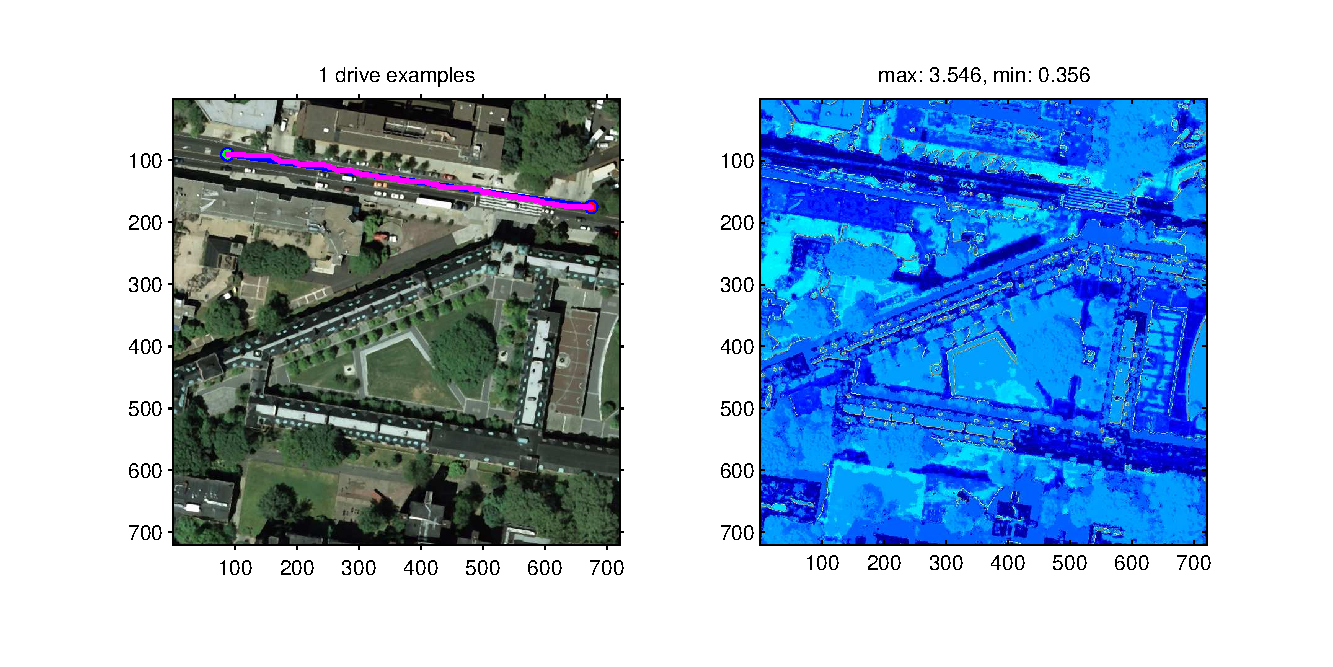
\includegraphics[width=\columnwidth]{fig/drive4.pdf}
\caption{drive4}
\label{fig:drive4}
\end{figure}

\begin{figure}[H]
\centering
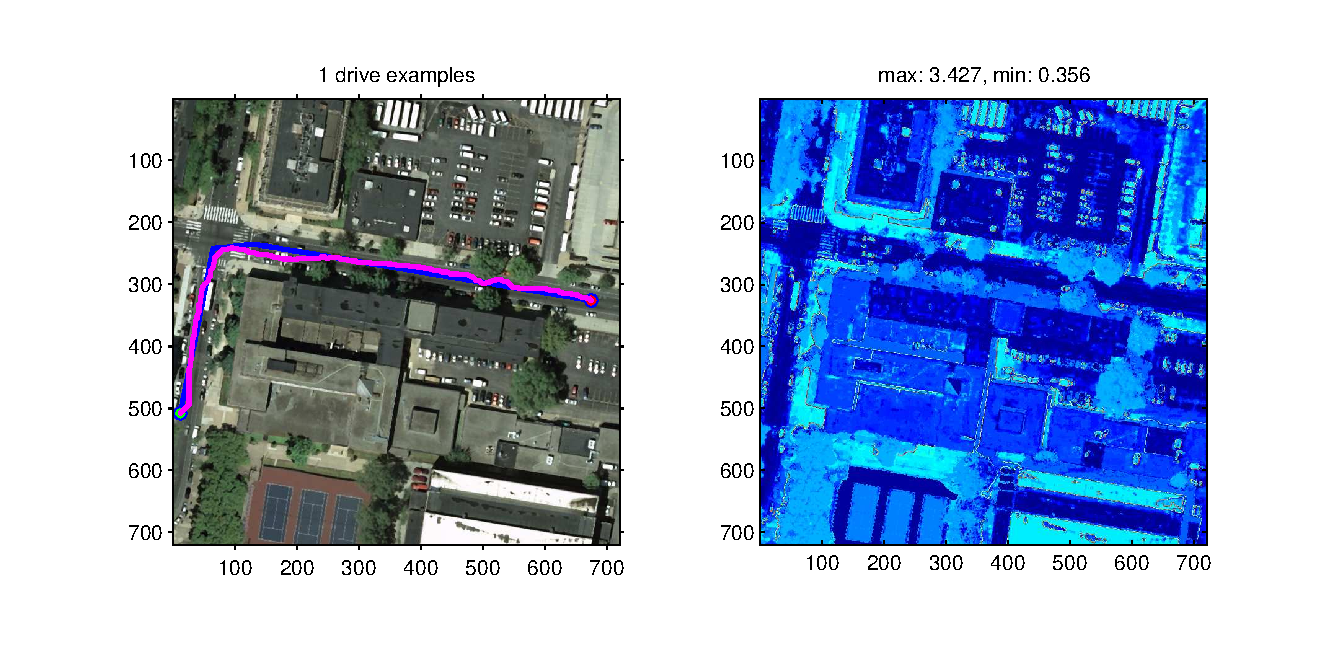
\includegraphics[width=\columnwidth]{fig/drive5.pdf}
\caption{drive5}
\label{fig:drive5}
\end{figure}

\begin{figure}[H]
\centering
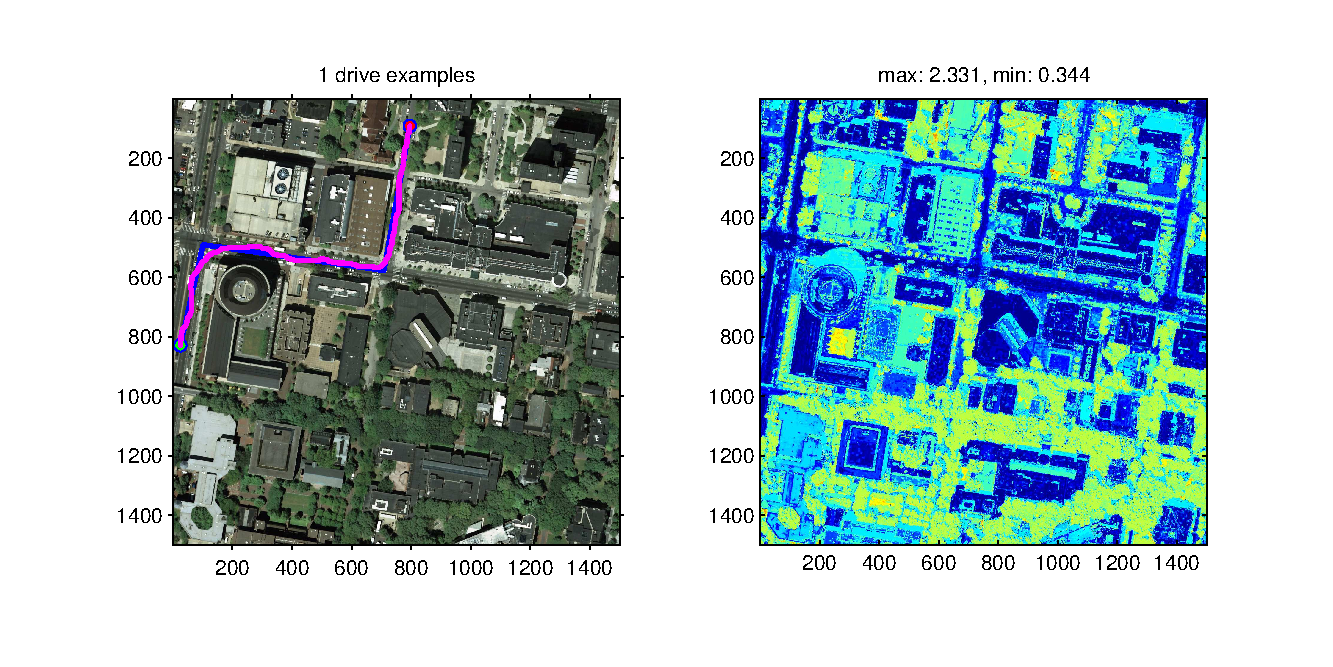
\includegraphics[width=\columnwidth]{fig/drive6.pdf}
\caption{drive6}
\label{fig:drive6}
\end{figure}

\begin{figure}[H]
\centering
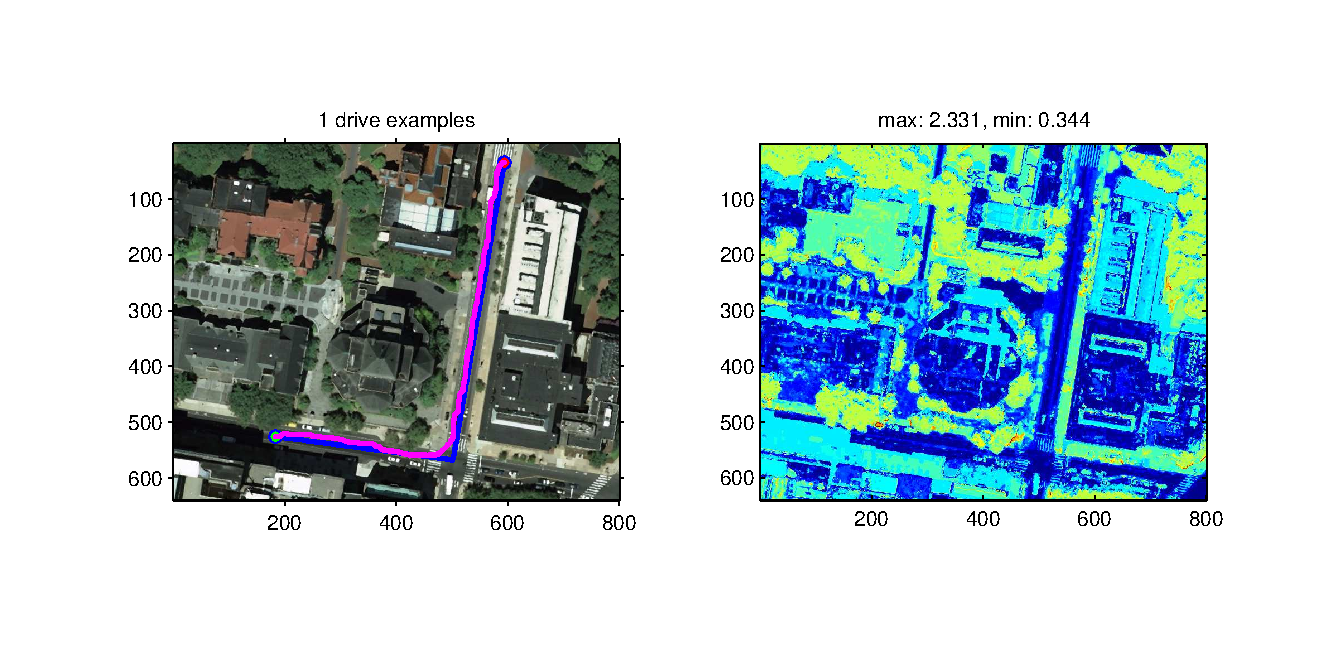
\includegraphics[width=\columnwidth]{fig/drive7.pdf}
\caption{drive7}
\label{fig:drive7}
\end{figure}
%-------------------------------------------------------------------------------
%	DISCUSSION
%-------------------------------------------------------------------------------

\section{Discussion}

%-------------------------------------------------------------------------------
%	REFERENCE LIST
%-------------------------------------------------------------------------------

\begin{thebibliography}{2} % Bibliography - this is intentionally simple in this template

%\bibitem{Vesa00}
%Vesa-Matti Mantyla, \emph{Hand gesture recognition of a mobile device user}. Multimedia and Expo, 2000. ICME 2000.
%
%\bibitem{Elmez07}
%Elmezain M. and Al-Hamadi A., \emph{A Hidden Markov Model-based continuous gesture recognition system for hand motion trajectory}. 19th International Conference on Pattern Recognition, ICPR 2008.
%
%\bibitem{Rabiner89}
%Lawrence R. Rabiner, \emph{A Tutorial on Hidden Markov Models and Selected Applications in Speech Recognition}. Proceedings of the IEEE, 1989.

\end{thebibliography}

%-------------------------------------------------------------------------------

\end{multicols}

\end{document}
